% \documentclass[margin=0mm]{standalone}
% \input{../tikz_header}


% \begin{document}





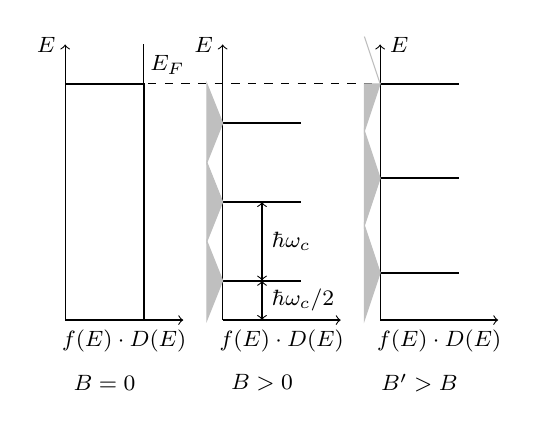
\begin{tikzpicture}[font=\footnotesize]
  %\useasboundingbox (0,0) rectangle (5,5);
  %\draw (11,10) rectangle ++(5,5);
  

  \draw[->] (0,0) -- ++ (0, 3.5) node[left] {$E$};
  \draw[->] (0,0) --   node[below] {$f(E) \cdot D(E)$} ++ (1.5, 0);
   \node at (0.5, -0.8) {$B=0$};

  \draw[thick] (1,0) -- (1,3) -- (0,3);
  \draw[thin] (1,0) -- (1,3.5);
  
  \draw[dashed] (0,3) -- (5,3);
   \node[above] at (1.3, 3) {$E_F$};

  %------ B > 0

  \draw[->] (2,0) -- ++ (0, 3.5) node[left] {$E$};
  \draw[->] (2,0) --   node[below] {$f(E) \cdot D(E)$} ++ (1.5, 0);
  \node at (2.5, -0.8) {$B>0$};

  \draw[thick] (2,0.5) -- ++ (1,0);
  \draw[thick] (2,1.5) -- ++ (1,0);
  \draw[thick] (2,2.5) -- ++ (1,0);

  \draw[<->] (2.5,0) -- node[right] {$\hbar \omega_c /2$} ++ (0,0.5) ;
  \draw[<->] (2.5,0.5) -- node[right] {$\hbar \omega_c $} ++ (0,1) ;

  
  \draw[lightgray,fill] (2,0.5) -- ++ (-0.2,0.5) -- ++ (0, -1) -- cycle;
  \draw[lightgray,fill] (2,1.5) -- ++ (-0.2,0.5) -- ++ (0, -1) -- cycle;
  \draw[lightgray,fill] (2,2.5) -- ++ (-0.2,0.5) -- ++ (0, -1) -- cycle;
 
    %------ B > B1 0
  
    \draw[->] (4,0) -- ++ (0, 3.5) node[right] {$E$};
    \draw[->] (4,0) --   node[below] {$f(E) \cdot D(E)$} ++ (1.5, 0);
    \node at (4.5, -0.8) {$B'>B$};
  
    \draw[thick] (4,0.6) -- ++ (1,0);
    \draw[thick] (4,1.8) -- ++ (1,0);
    \draw[thick] (4,3.0) -- ++ (1,0);
    
    
    \draw[lightgray,fill] (4,0.6) -- ++ (-0.2,0.6) -- ++ (0, -1.2) -- cycle;
    \draw[lightgray,fill] (4,1.8) -- ++ (-0.2,0.6) -- ++ (0, -1.2) -- cycle;
    \draw[lightgray,fill] (4,3.0) -- ++ (-0.2,-0.6) -- ++ (0, 0.6) -- cycle;
    \draw[lightgray] (4,3.0) -- ++ (-0.2,+0.6) ;
   
  
\end{tikzpicture}

%\end{document}